\section{Detecting DNS Amplification Attacks with Zeek}
Zeek stands out as a powerful network security tool, capable of real-time monitoring and analysis of network traffic. It is particularly effective in detecting and mitigating DNS Amplification attacks, a type of Distributed Denial of Service (DDoS) attack that leverages public DNS servers to overwhelm a target with disproportionate DNS response traffic.
\subsection{How It Works}
The following points outline Zeek's approach to identifying DNS Amplification attacks:

\begin{enumerate}
    \item \textbf{Monitoring DNS Traffic}: Zeek meticulously observes network traffic, focusing on DNS activities to capture both query requests and their responses, thereby monitoring the exchanges between clients and DNS servers.
    
    \item \textbf{Analyzing Response Sizes}: Zeek assesses the size of DNS response packets, identifying potential amplification behavior when response sizes significantly exceed those of the query requests.
    
    \item \textbf{Establishing Baseline Metrics}: Zeek establishes baseline metrics for standard DNS traffic, including typical sizes for requests and responses and normal query rates, which assists in spotting deviations that might indicate an attack.
    
    \item \textbf{Threshold Configuration}: Within Zeek's configuration, customizable thresholds are set for factors such as response size limits and query rate caps. Surpassing these thresholds may indicate a potential DNS Amplification attack.
    
    \item \textbf{Pattern Recognition}: Zeek detects patterns that align with DNS Amplification characteristics, like an unusual influx of large response packets directed at a single target or increased queries to open DNS resolvers.
    
    \item \textbf{Incident Logging and Alerts}: When Zeek identifies anomalies consistent with DNS Amplification attacks, it logs the incidents and can also be configured to issue real-time alerts, facilitating prompt intervention and attack mitigation.
\end{enumerate}
\subsection{DNS Script :}
\begin{lstlisting}[language=Python, caption=]
@load base/protocols/dns

module Notice;

export {
    redef enum Notice::Type += {DNS_Amplification_Suspected};
}
global dns_query_threshold: count = 20;
global suspicious_dns_activity: table[addr] of count = {};

event dns_request(c: connection, msg: dns_msg, query: string, qtype: count, qclass: count) {
    local src = c$id$orig_h;
    if ( src in suspicious_dns_activity ) {
        suspicious_dns_activity[src] += 1;
    } else {
        suspicious_dns_activity[src] = 1;
    }

    if ( suspicious_dns_activity[src] > dns_query_threshold ) {
        NOTICE([$note=DNS_Amplification_Suspected,
                $msg=fmt("High volume of DNS requests from %s, potential DNS Amplification.", src),
                $src=src,
                $conn=c]);
                
        delete suspicious_dns_activity[src];
    }
}

event dns_query_reply(c: connection, msg: dns_msg, query: string, qtype: count, qclass: count) {
    local src = c$id$orig_h;
    if ( src in suspicious_dns_activity ) {
        suspicious_dns_activity[src] += 1;
    } else {
        suspicious_dns_activity[src] = 1;
    }

    if ( suspicious_dns_activity[src] > dns_query_threshold ) {
        NOTICE([$note=DNS_Amplification_Suspected,
                $msg=fmt("High volume of DNS requests from %s, potential DNS Amplification.", src),
                $src=src,
                $conn=c]);
                
        delete suspicious_dns_activity[src];
    }
}
\end{lstlisting}
\subsection{DNS Script Explanation}


\begin{enumerate}
    
    \item \textbf{DNS Script Inclusion} (Line 1): The script initiates by incorporating DNS protocol analysis functionalities through `\texttt{@load base/protocols/dns}`, enabling inspection of DNS traffic.

    \item \textbf{Notice Module Extension} (Lines 2-6): The script enhances the `\texttt{Notice}` module by appending a new notice type called `\texttt{DNS\_Amplification\_Suspected}`, designed for alerting upon detection of suspicious DNS activities.

    \item \textbf{Global Variables Declaration} (Lines 8-9):
    \begin{itemize}
        \item `\texttt{dns\_query\_threshold}`: Sets a threshold (20 in this context) to delineate the normal count of DNS queries from a single IP before it is deemed suspicious.
        \item `\texttt{suspicious\_dns\_activity}`: Initializes a table to record the number of DNS queries made by each source IP address, facilitating the tracking of DNS request frequencies.
    \end{itemize}

    \item \textbf{DNS Request Event Handling} (\texttt{dns\_request})(Lines 11-27):
    \begin{itemize}
        \item The script monitors `\texttt{dns\_request}` events, triggered by DNS queries.
        \item Extracts the source IP (`\texttt{src}`) from each DNS request's connection details.
        \item Updates the `\texttt{suspicious\_dns\_activity}` table with the query count for the source IP, adding the IP with a count of 1 if it's not already present.
        \item Generates a `\texttt{DNS\_Amplification\_Suspected}` notice if the query count for a source IP surpasses the `\texttt{dns\_query\_threshold}`, indicating potential DNS amplification attack behavior.
        \item Resets the query count for the source IP in the `\texttt{suspicious\_dns\_activity}` table by removing its entry post-notice generation to avoid repetitive alerts.
    \end{itemize}


  \item \textbf{DNS Query Reply Event (\texttt{dns\_query\_reply})  (Lines 29-45):}
  \begin{itemize}
    \item Triggered for each DNS query reply observed in the monitored traffic.
    \item Increments a counter in \texttt{suspicious\_dns\_activity} for the source IP address of the query (\texttt{c\$id\$orig\_h}).
    \item If the count for an IP address exceeds \texttt{dns\_query\_threshold}, a \texttt{DNS\_Amplification\_Suspected} notice is generated, indicating potential amplification activity from that IP address.
    \item The entry for the IP address in \texttt{suspicious\_dns\_activity} is deleted after generating the notice, resetting its count.
  \end{itemize}


\end{enumerate}


\subsection{Simulation :}
Here is the link to PCAP file:
\href{https://www.malware-traffic-analysis.net/tutorials/index.html}{malware-traffic-analysis}\\\\
\begin{itemize}
    \item The process starts by analyzing a PCAP file with dns.zeek, which uses DNS protocol analysis to detect potential DNS Amplification attacks by identifying abnormal DNS query volumes, defining a specific notice type DNS\_Amplification\_Suspected for such events.
\end{itemize}

\begin{figure}[H]
    \centering
    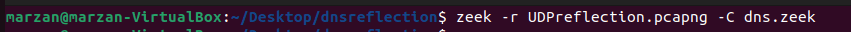
\includegraphics[width=1\linewidth]{images//UDP_reflection/udp_3.png}
    \caption{Script Execution}
    \label{fig:enter-label}
\end{figure}

\begin{itemize}
    \item The notice.log entries indicate the IP 198.51.100.165's excessive DNS requests, suggesting potential DNS Amplification attacks. These entries document the incident details, including the involved IPs and ports, and mark each event for logging with a one-hour suppression to mitigate repeat alerts.
\end{itemize}
\begin{figure}[H]
    \centering
    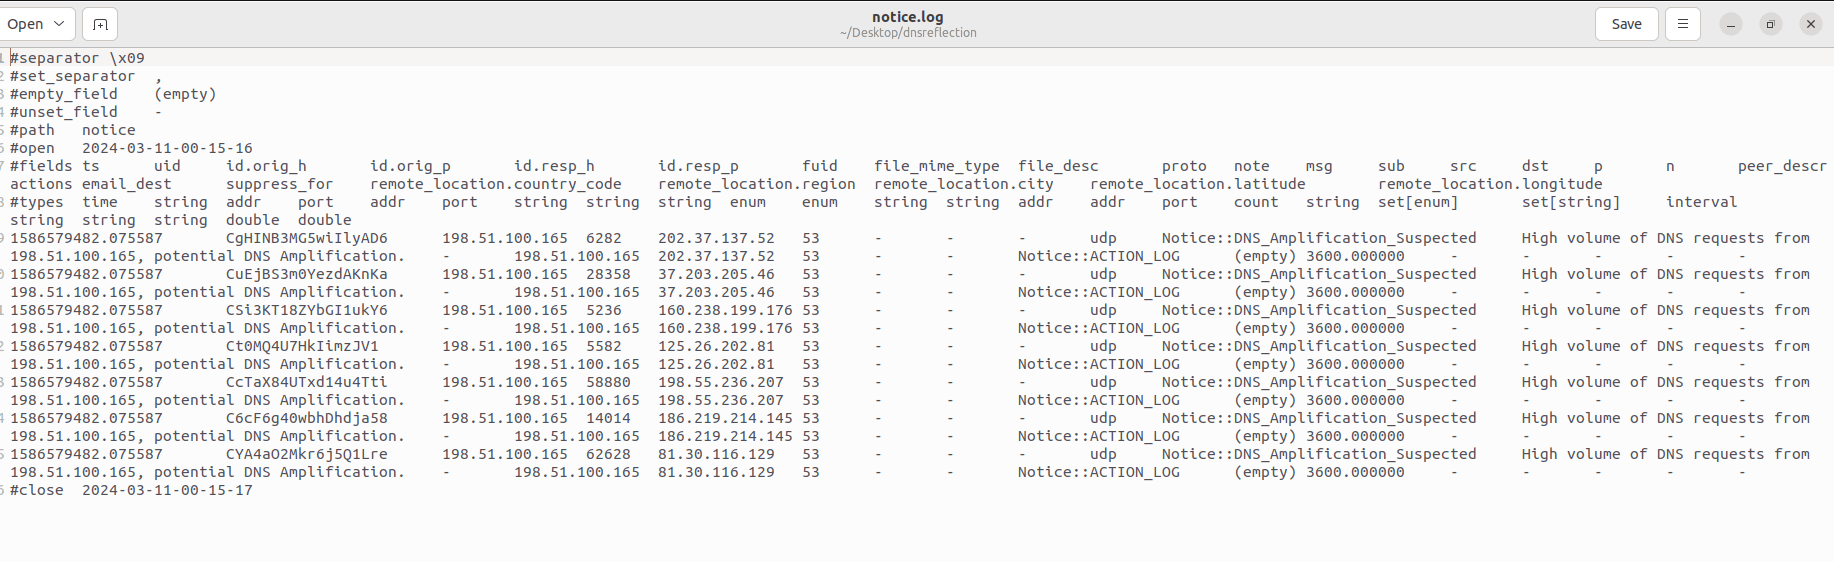
\includegraphics[width=1\linewidth]{images//UDP_reflection/udp_4.png}
    \caption{notice.log}
    \label{fig:enter-label}
\end{figure}

\begin{itemize}
    \item In BRIM, the notice.log is organized into a formal tabular representation, systematically displaying instances of potential DNS Amplification attacks originating from the IP 198.51.100.165.
\end{itemize}
\begin{figure}[H]
    \centering
    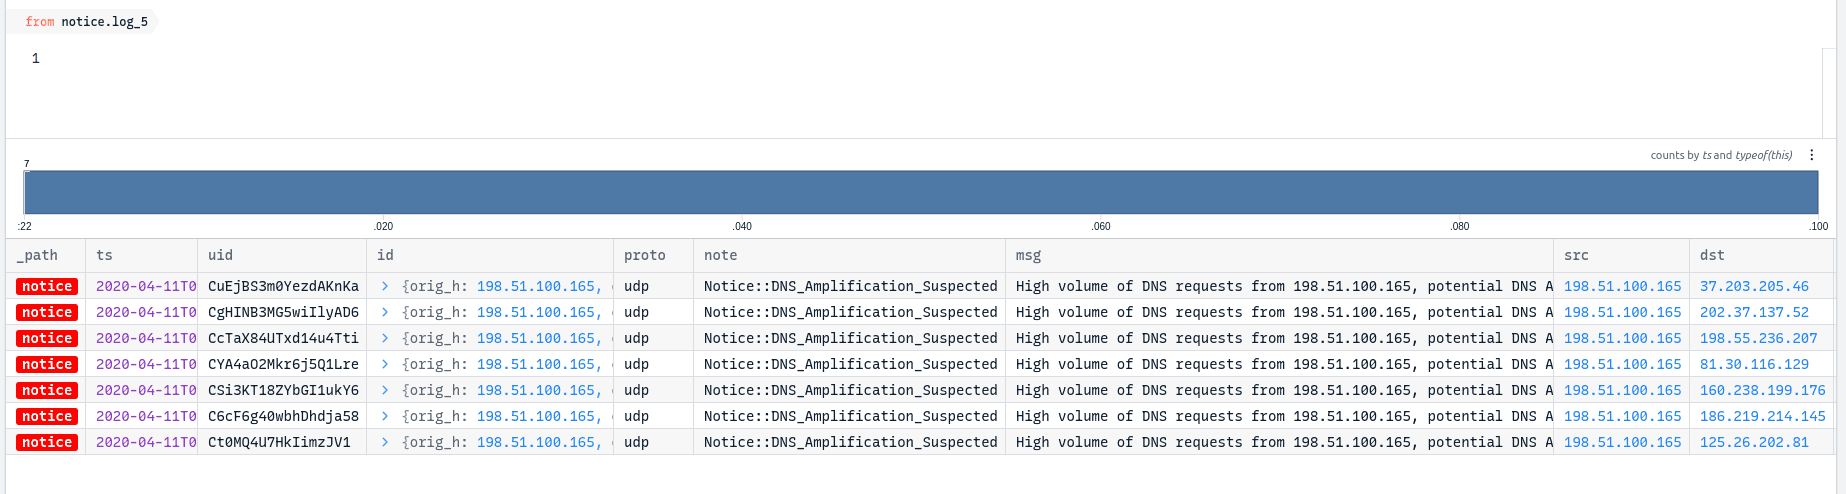
\includegraphics[width=0.8\linewidth]{images//UDP_reflection/udp_5.png}
    \caption{notice.log in BRIM}
    \label{fig:enter-label}
\end{figure}






\subsection{Example Script :}
\begin{lstlisting}[language=Python, caption=]
module DDosAttacks;
@load base/protocols/dns

redef enum Notice::Type += {
    DNSDDoSAmplification
};

function generate_ddos_notice(c: connection, query: string) {
    local query1: string = strip(query);
    if (query1 == "peacecorps.gov" || query1 == "pizzaseo.com") {
        NOTICE([$note = DNSDDoSAmplification,
            $msg = fmt("Possible DNS DDoS Amplification Attack"),
            $conn = c,
            $uid = c$uid
        ]);
    }
}

event dns_request(c: connection, msg: dns_msg, query: string, qtype: count, qclass: count, original_query: string) {
    generate_ddos_notice(c, query);
}

event dns_query_reply(c: connection, msg: dns_msg, query: string, qtype: count, qclass: count, original_query: string) {
    generate_ddos_notice(c, query);
}
\end{lstlisting}

\subsection{Example Script Explanation}

\begin{enumerate}
    
    \item \textbf{Module Declaration and DNS Script Loading} (Lines 1-2): The script commences with the declaration of a module titled `DDosAttacks`. It proceeds to integrate DNS protocol analysis functionalities from the Zeek standard library through the command `\texttt{@load base/protocols/dns}`.

    \item \textbf{Enumeration Extension for Notice} (Lines 4-5): The script enhances the `\texttt{Notice::Type}` enumeration by appending a novel type named `DNSDDoSAmplification`. This addition is aimed at facilitating the signaling of potential DNS DDoS amplification attacks.

    \item \textbf{DDoS Notice Generation Function} (Lines 8-17): A function named `\texttt{generate\_ddos\_notice}` is introduced. It is designed to examine network connections (denoted as `c`) and DNS queries (denoted as `query`). The function scrutinizes the DNS query after removing any whitespace and, if it matches specific domains (`peacecorps.gov` or `pizzaseo.com`), it issues a notice of type `DNSDDoSAmplification`.

    \item \textbf{DNS Request Event Handling} (Lines 19-21): The script configures an event handler named `\texttt{dns\_request}`. This handler is triggered for every DNS request and it invokes the `\texttt{generate\_ddos\_notice}` function. This mechanism is employed to assess each DNS inquiry for indications of DNS DDoS amplification attacks.

    \item \textbf{DNS Query Reply Event Handling} (Lines 23-25): Similarly, the script sets up another event handler named `\texttt{dns\_query\_reply}`. This handler also calls the `\texttt{generate\_ddos\_notice}` function for DNS responses, thereby extending the surveillance to include reply messages which might be pertinent in detecting attack patterns.
\end{enumerate}

\subsection{Simulation :}
Here is the link to PCAP file:
\href{https://www.malware-traffic-analysis.net/tutorials/index.html}{malware-traffic-analysis}\\\\
\begin{itemize}
    \item  The process begins with the execution of a PCAP file through the example.zeek script, part of the DDosAttacks module, which loads DNS protocol analyses. The script is designed to identify potential DNS DDoS Amplification attacks by inspecting DNS queries. If a query matches specific target domains, it triggers a DNSDDoSAmplification notice.
\end{itemize}
\begin{figure}[H]
    \centering
    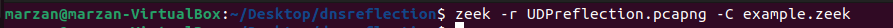
\includegraphics[width=1\linewidth]{images//UDP_reflection/udp_1.png}
    \caption{Script Execution}
    \label{fig:enter-label}
\end{figure}

\begin{itemize}
    \item The resulting notice.log entries, visualized in BRIM in a tabular format, detail instances where the script detected potential DNS DDoS Amplification attacks. Each entry includes the timestamp, source and destination IP addresses and ports, protocol used (UDP), and a message indicating a "Possible DNS DDoS Amplification Attack". The action logged is Notice::ACTION\_LOG, and a suppression period of 3600 seconds is set to prevent immediate duplicate alerts.
\end{itemize}
\begin{figure}[H]
    \centering
    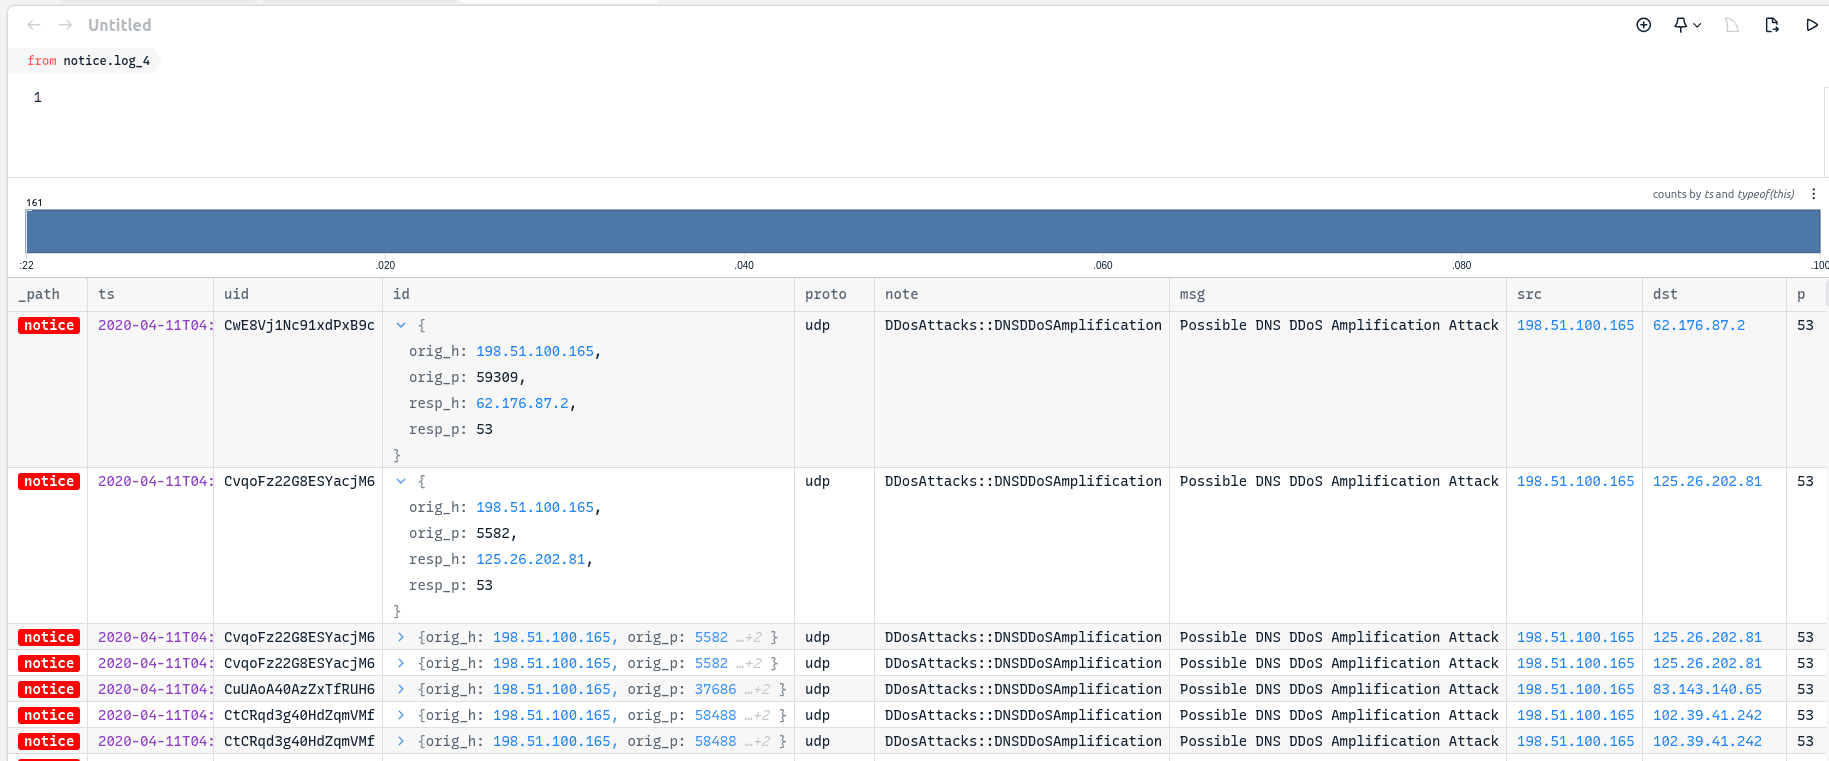
\includegraphics[width=1\linewidth]{images//UDP_reflection/udp_2.png}
    \caption{notice.log Analysis in BRIM}
    \label{fig:enter-label}
\end{figure}

